%! Author = ahmed_hassanien
%! Date = 3/21/20

% Preamble
\documentclass[aspectratio=169]{beamer}
%%% TOC
%%% 1. Introduction & What is the problem with the current deployment process? Why do we need to enhance it?
%%% 2. What is virtualization? vistual vs physical? slide number 6 to be splitted.
%%% What do we mean by islolation? What is the different type of virtualization linux? win? mac?
%%% 3. What is Hypervisor? Why do we need it? Is there any difference between it in windows, linux, and mac?
%%% Does the same concept implemented into the same why in all OSs?
%%% 4. Containerization? What is containerization? Containerization Historical thoery? Where can we find it? what is the relation between it and (VM, OS, Hardware)?
%%% Can we have containerization for windows and mac and linux, if no why?
%%% Why do we need containerization with CICD? Why it is important?
%%% What do you mean by kernal?
% Packages
\usepackage[sectionpage=progressbar,progressbar=foot]{theme/beamerthememetropolis}
\usepackage{tikz}
\tikzset{
    invisible/.style={opacity=0},
    visible on/.style={alt={#1{}{invisible}}},
    alt/.code args={<#1>#2#3}{%
        \alt<#1>{\pgfkeysalso{#2}}{\pgfkeysalso{#3}} % \pgfkeysalso doesn't change the path
    },
}
% Libraries
\usetikzlibrary{positioning}

% Details
\title{Containerization \& Virtualization}
\date{\today}
\author{Ahmed Hassanien}
\institute{Garage Education}

% Document
\begin{document}
    \maketitle

    \begin{frame}{Table of contents}
        \setbeamertemplate{section in toc}[sections numbered]
        \tableofcontents[hideallsubsections]
    \end{frame}

    %----------------------------------------------------------------------------------------------------------------------%

\section{Introduction - Docker Overview}\label{sec:introduction-docker-overview}
%----------------------------------------------------------------------------------------------------------------------%

\subsection{What is docker?}\label{subsec:what-is-docker}
\begin{frame}{What is docker?}
    \begin{itemize}[<+- | alert@+>]
        \item Docker is an OS-level virtualization tool.
        \item Docker is an open platform for developing, shipping, and running applications.
        \item Docker provides tools, and a platform to manage the lifecycle of your containers:
        \begin{itemize}
            \item Develop your application and its supporting components using containers.
            \item The container becomes the unit for distributing and testing your application.
            \item When you are ready, deploy your application into your production environment, as a container or an orchestrated service.
            \item This works the same whether your production environment is a local data center, a cloud provider, or a hybrid of the two.
        \end{itemize}
    \end{itemize}
\end{frame}

\subsection{Docker Architecture}\label{subsec:docker-architecture}
\begin{frame}{Docker Architecture}
    \begin{itemize}
        \item Docker uses a client-server architecture.
        \linebreak
        \pause
        \begin{figure}[!t]
            \raggedright
            \begin{tikzpicture}[
    node/.style = {
        scale=0.70,
        node distance = 2mm,
        rectangle,
        draw = black,
        thick,
        text centered,
        minimum height = 10mm,
        minimum width = 10mm
    },
    txt/.style = {
        scale=0.70,
        node distance = 2mm,
        rectangle,
        text centered,
        minimum height = 2mm,
        minimum width = 10mm
    }
]
    \tikzstyle{layer} = [inner sep=1mm, draw=black, thick, fill= gray!30]
    \tikzstyle{vm} = [fill = gray!30]
    \tikzstyle{hw} = [fill = blue!35]
    \tikzstyle{sw} = [fill = blue!15]
    \tikzstyle{hv} = [fill = blue!5 ]
    \tikzstyle{ar} = [fill = black  ]

    %%%%%%%%%%%%%%%%%
    % Docker Client %
    %%%%%%%%%%%%%%%%%
    \node [txt, text width=3cm, visible on=<1->] (CLIENT) {Client};
    \node [node, hw, above = of CLIENT, text width=3cm, visible on=<3->] (REST) {Rest};
    \node [node, hw, above = of REST, text width=3cm, visible on=<4->] (CLI) {CLI};
    \begin{scope}[on background layer]
        \node [fit = (CLIENT) (REST) (CLI), layer, visible on=<1->] {};
    \end{scope}

    %%%%%%%%%%%%%%%%%
    % Docker Server %
    %%%%%%%%%%%%%%%%%
    \node [txt, right = of CLIENT, text width=4cm, xshift = 2mm, visible on=<5->] (SER) {Server - Docker Demon};
    \node [node, hw, above = of SER, text width=4cm, visible on=<6->] (IMG) {Images};
    \node [node, hw, above = of IMG, text width=4cm, visible on=<7->] (CON) {Containers};
    \node [node, hw, above = of CON, text width=4cm, visible on=<8->] (VOL) {Volumes};
    \begin{scope}[on background layer]
        \node [fit = (SER) (CON) (IMG) (VOL), layer, visible on=<5->] {};
    \end{scope}

    %%%%%%%%%%%%%%%%%%%
    % Docker Rigestry %
    %%%%%%%%%%%%%%%%%%%
    \node [txt, right = of SER, text width=3cm, xshift = 2mm, visible on=<9->] (REG) {Registry};
    \node [node, hw, above = of REG, text width=3cm, visible on=<10->] (HUB) {Docker Hub};
    \begin{scope}[on background layer]
        \node [fit = (REG) (HUB), layer, visible on=<9->] {};
    \end{scope}
\end{tikzpicture}
            \caption{Docker Architecture}
        \end{figure}
    \end{itemize}
\end{frame}
\begin{frame}{Docker Demon (Server)}
    \begin{itemize}[<+- | alert@+>]
        \item The Docker daemon \texttt{(dockerd)} listens for Docker API requests and manages Docker objects.
        \item A daemon can also communicate with other daemons to manage Docker services.

    \end{itemize}
\end{frame}
\begin{frame}{Docker Objects}
    \begin{itemize}[<+- | alert@+>]
        \item \textbf{Images} are a read-only template with instructions for creating a Docker container.
        \item \textbf{Containers} are a runnable instance of an image.
        \item \textbf{Volumes} are the preferred mechanism for persisting data generated by and used by Docker containers.
    \end{itemize}
\end{frame}
\begin{frame}{Docker Client}
    \begin{itemize}[<+- | alert@+>]
        \item The Docker client \texttt{(docker)} is the primary way that many Docker users interact with Docker.
        \item When you use commands such as \texttt{(docker run)}, the client sends these commands to \texttt{(dockerd)}, which carries them out.
        \item The docker command uses the Docker API and can communicate with one or more docker daemons.
    \end{itemize}
\end{frame}
\begin{frame}{Docker Registry}
    \begin{itemize}[<+- | alert@+>]
        \item A Docker registry stores Docker images.
        \item Docker Hub is a public registry that anyone can use, and by default Docker configurations looks for the images on Docker Hub.
        \item Docker Hub is not the only registry in the market, and you can use your own docker registry.
    \end{itemize}
\end{frame}
%----------------------------------------------------------------------------------------------------------------------%
    %----------------------------------------------------------------------------------------------------------------------%


\section{Virtualization}\label{sec:virtualization}
%----------------------------------------------------------------------------------------------------------------------%

\subsection{Virtual Machines}\label{subsec:virtual-machines}
\begin{frame}{Virtual Machines}
    \begin{itemize}
        \item Virtual machines (VMs) are an abstraction of physical hardware.
        \item It allows you to run multiple Virtual Machines (VMs) on a single physical server's CPU\@.
        \item Each VM includes a full copy of an operating system, the application, necessary binaries, and libraries - taking up tens of GBs.
        \item Virtualization allows applications to be isolated between VMs.
        \item Virtualization provides a level of security as the information of one application cannot be freely accessed by another application.
        \item Virtualization allows better utilization of resources in a physical server.
        \item Virtualization allows better scalability because an application can be added or updated easily,
        \item Virtualization reduces hardware costs, and much more.
        \item Virtualization can present a set of physical resources as a cluster of disposable virtual machines.
    \end{itemize}
\end{frame}

\subsection{Virtualized Deployment}\label{subsec:virtualized-deployment}
\begin{frame}{Virtualized Deployment}
    PICTURE GOES HERE
\end{frame}

\subsection{Hypervisor}\label{subsec:hypervisor}
\begin{frame}{Hypervisor}
    \begin{itemize}
        \item How virtualization is possible?
        \begin{itemize}
            \item A hypervisor is computer software, firmware or hardware that creates and runs virtual machines.
            \item The hypervisor allows multiple VMs to run on a single machine.
        \end{itemize}
        \item It is usually classified to 2 types:
        \begin{itemize}
            \item Type-1, native or bare-metal hypervisors .
            \item Examples: VMware ESX and Citrix Xen servers.
            \item Type-2 or hosted hypervisors
            \item Examples: VMware player and VirtualBox.
        \end{itemize}
        \item PICTURES GOES HERE
    \end{itemize}
\end{frame}
%----------------------------------------------------------------------------------------------------------------------%
    
%---------------------------------------------------------
\section{Containerization}
%---------------------------------------------------------

%---------------------------------------------------------
\subsection{History of running a software}
\begin{frame}
	\frametitle{History of running a software}
	\begin{itemize}
		\item Install or use an existing operating system.
		\item Install the tools used by your software.
		\item Install dependencies of your software.
		\item Run your software.
		\item Repeat or reuse for every new software version release.
	\end{itemize}
\end{frame}
%---------------------------------------------------------

%---------------------------------------------------------
\subsection{Issues and motive behind containerization}
\begin{frame}
	\frametitle{Issues and motive behind containerization}
	\begin{itemize}
		\item Containerization eliminates the quote, "it worked on my machine." (\textbf{Low risk of failing in production}).
		\item Containerization eliminates the installation and configuration time. (\textbf{Easy and fast deployment}).
		\item Containerization packages Software into Standardized Units for Development, Shipment, and Deployment. (\textbf{Isolation}).
		\item Containerization eliminates infrastructure wasted resources and utilizes them.
		\item Containerization easy the scalability dilemma.
	\end{itemize}
\end{frame}
%---------------------------------------------------------

%---------------------------------------------------------
\subsection{What is a Container?}
\begin{frame}
	\frametitle{What is a Container?}
	\begin{itemize}
		\item A standardized unit of software.
		\item A container packages up code and all its dependencies, so the application runs quickly and reliably from one computing environment to another.
		\item A container image is a lightweight, standalone, executable package of software that includes everything needed to run an application: 
		\begin{itemize}
			\item code, 
			\item runtime, 
			\item system tools, 
			\item system libraries 
			\item and settings.
		\end{itemize}
	\end{itemize}
\end{frame}
%---------------------------------------------------------

%---------------------------------------------------------
\subsection{Containers VS Virtual Machines}
\begin{frame}
	\frametitle{Containers VS Virtual Machines}
	Containers and virtual machines have similar resource isolation and allocation benefits but function in a  different way. Containers virtualize the operating system instead of hardware, and they are more portable and efficient.
	\linebreak
	
	\centering
	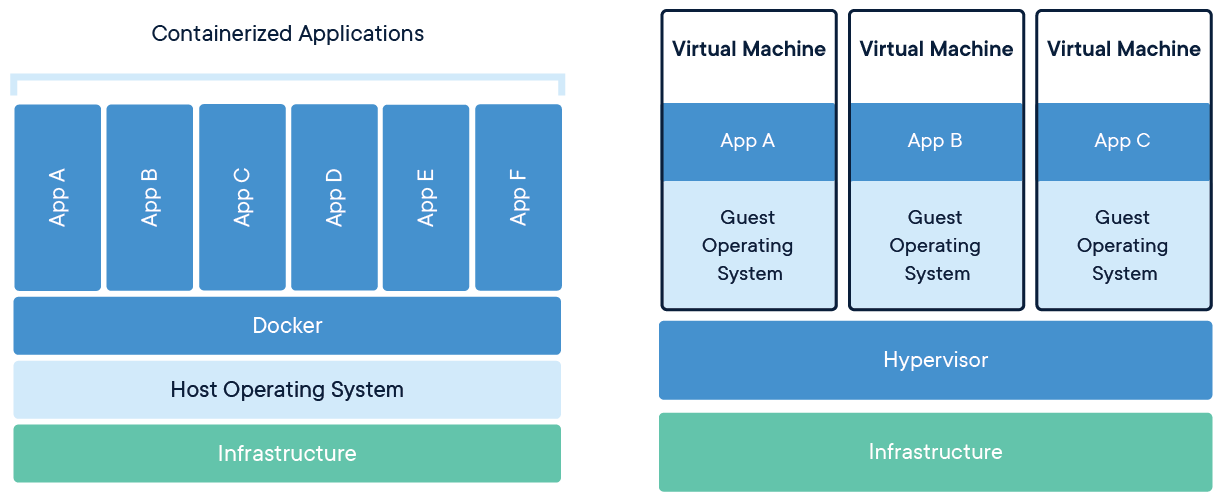
\includegraphics[width=\linewidth]{figures/docker-containerized-and-vm-transparent-bg.png}
\end{frame}
%---------------------------------------------------------

%---------------------------------------------------------
\subsection{Virtual Machines}
\begin{frame}
	\frametitle{Virtual Machines}
	\begin{itemize}
		\item Virtual machines (VMs) are an abstraction of physical hardware, turning one server into many servers.
		\item The hypervisor allows multiple VMs to run on a single machine.
		\item Each VM includes a full copy of an operating system, the application, necessary binaries, and libraries - taking up tens of GBs.
		\item VMs can also be slow to boot.
	\end{itemize}
\end{frame}
%---------------------------------------------------------

%---------------------------------------------------------
\subsection{Containers}
\begin{frame}
	\frametitle{Containers}
	\begin{itemize}
		\item Containers are an abstraction at the app layer that packages code and dependencies together.
		\item Multiple containers can run on the same machine and share the OS kernel with other Containers, each running as isolated processes in userspace.
		\item Containers take up less space than VMs (container images are typically tens of MBs in size), can handle more applications, and require fewer VMs and Operating systems. 
	\end{itemize}
\end{frame}
%---------------------------------------------------------

%---------------------------------------------------------
\subsection{Container-based virtualization Solutions}
\begin{frame}
	\frametitle{Container-based virtualization Solutions}
	\begin{itemize}
		\item \textbf{Docker} is the most popular, and we will explain briefly.
		\item \textbf{OpenVZ}
		\item \textbf{LXC} Linux containers 
	\end{itemize}
\end{frame}
%---------------------------------------------------------

%---------------------------------------------------------
\subsection{References}
\begin{frame}
	\frametitle{References}
	\begin{itemize}
		\item \href{https://www.docker.com/resources/what-container}{Docker - What is a container?}
		\item \href{https://openvz.org/}{OpenVZ}
		\item \href{https://linuxcontainers.org/}{Linux Containers}
	\end{itemize}
\end{frame}
%---------------------------------------------------------

    %----------------------------------------------------------------------------------------------------------------------%


\section{Summary and Popular Questions}\label{sec:popular-questions}
%----------------------------------------------------------------------------------------------------------------------%

\subsection{Summary}\label{subsec:summary}
\begin{frame}
    \begin{itemize}[<+- | alert@+>]
        \item The word virtualization applies to hardware and operating system.
        \item Hardware virtualization produces virtual machines.
        \item Operating system virtualization produces containers.
    \end{itemize}
\end{frame}

\subsection{Why Containers are more popular?}\label{subsec:containers-are-more-popular}
\begin{frame}{Why Containers are more popular?}
    \begin{itemize}[<+- | alert@+>]
        \item Containerization gives us better resource isolation with predictable application performance.
        \item Containerization gives us better resource utilization with high efficiency and density.
        \item They are loosely coupled, distributed, elastic, liberated micro-services.
        \item Environmental consistency across development, testing, and production \textbf{"It worked on my machine."}
        \item Agile application creation and deployment.
    \end{itemize}
\end{frame}

\subsection{What is hybrid container architecture?}\label{subsec:what-is-hybrid-container-architecture?}
\begin{frame}{What is hybrid container architecture?}
    \begin{itemize}[<+- | alert@+>]
        \item A hybrid container architecture is an architecture combining virtualization on both hardware and OS levels.
        \item Example: The container engine and associated containers execute on top of a virtual machine.
        \item Use of a hybrid container architecture is also known as hybrid containerization.
    \end{itemize}
\end{frame}

\subsection{Hybrid container architecture}\label{subsec:hybrid-container-architecture}
\begin{frame}{Hybrid container architecture}
    \begin{figure}[!t]
        \raggedright
        \begin{tikzpicture}[
            node/.style={
                scale=0.60,
                node distance = 2mm,
                rectangle,
                draw = black,
                thick,
                text centered,
                minimum height = 10mm,
                minimum width = 10mm
            },
            txt/.style = {
                scale = 0.60,
                node distance = 2mm,
                rectangle,
                text centered,
                minimum height = 2mm,
                minimum width = 10mm
            }
        ]
            \tikzstyle{layer} = [inner sep=1mm, draw=black, thick, fill= gray!30]
            \tikzstyle{vm} = [fill = gray!30]
            \tikzstyle{hw} = [fill = blue!35]
            \tikzstyle{sw} = [fill = blue!15]
            \tikzstyle{hv} = [fill = blue!5 ]

            %%%%%%%%%%%%%%%%%%%%%%%%%%%%%%%%%
            % Hybrid container architecture %
            %%%%%%%%%%%%%%%%%%%%%%%%%%%%%%%%%
            \node [node, hw, text width=10cm, yshift=-2mm, visible on=<1->] (HW) {Hardware};
            \node [node, hv, above = of HW, text width=10cm, yshift=-2mm, visible on=<2->] (HV1) {Hypervisor};
            \node [node, sw, above = of HV1, text width=10cm, yshift=-2mm, visible on=<3->] (OS1) {Host Operating System};
            % Virtual Machine 1
            \node [txt , vm, above = of OS1, text width=4.35cm, xshift = -2.60cm, visible on=<4->] (VM1) {Virtual Machine};
            \node [node, sw, above = of VM1, text width=4.45cm, yshift=-2mm, visible on=<5->] (OS2) {Guest OS};
            \node [node, hv, above = of OS2, text width=4.45cm, yshift=-2mm, visible on=<6->] (HV2) {Container Runtime};
            \node [node , sw, above = of HV2, text width=1.13cm, yshift=-2mm, xshift = -1.65cm, visible on=<7->] (CO1) {C1};
            \node [node , sw, right = of CO1, text width=1.13cm, xshift = -1mm, visible on=<8->] (CO2) {C2};
            \node [node , sw, right = of CO2, text width=1.13cm, xshift = -1mm, visible on=<9->] (CO3) {C3};
            \begin{scope}[on background layer]
                \node [fit = (VM1) (OS2) (HV2) (CO1) (CO2) (CO3), layer, visible on=<4->] {};
            \end{scope}
            % Virtual Machine 2
            \node [txt , right = of VM1, text width=4.45cm, xshift = 2mm, visible on=<10->] (VM2) {Virtual Machine};
            \node [node, sw, above = of VM2, text width=4.45cm, yshift=-2mm, visible on=<10->] (OS3) {Guest OS};
            \node [node, hv, above = of OS3, text width=4.45cm, yshift=-2mm, visible on=<10->] (HV3) {Container Runtime};
            \node [node , sw, above = of HV3, text width=1.13cm, yshift=-2mm, xshift = -1.65cm, visible on=<10->] (CO4) {C1};
            \node [node , sw, right = of CO4, text width=1.13cm, xshift = -1mm, visible on=<10->] (CO5) {C2};
            \node [node , sw, right = of CO5, text width=1.13cm, xshift = -1mm, visible on=<10->] (CO6) {C3};
            \begin{scope}[on background layer]
                \node [fit = (VM2) (OS3) (HV3) (CO4) (CO5) (CO6), layer, visible on=<10->] {};
            \end{scope}
        \end{tikzpicture}
        \caption{Hybrid container architecture}
    \end{figure}
\end{frame}

\subsection{Do windows have native containers?}\label{subsec:windows-containers}
\begin{frame}{Do windows have native containers?}
    \begin{itemize}[<+- | alert@+>]
        \item You can have native windows containers but not Linux native containers yet.
        \item Microsoft's native hypervisor solution is Hyper-V\@.
        \item Using Hyper-V Microsoft supports running VMs natively on Windows, for example, Ubuntu on Windows (WSL).
        \item Microsoft is working on the OS-level virtualization solution to run Linux native containers.
    \end{itemize}
\end{frame}
%----------------------------------------------------------------------------------------------------------------------%
    %----------------------------------------------------------------------------------------------------------------------%


\section{References}\label{sec:references}
%----------------------------------------------------------------------------------------------------------------------%

\begin{frame}{References}
    \begin{itemize}
        \item \href{https://insights.sei.cmu.edu/sei_blog/2017/09/virtualization-via-containers.html}{Virtualization via containers}
        \item \href{https://en.wikipedia.org/wiki/OS-level_virtualization}{OS-level virtualization}
        \item \href{https://en.wikipedia.org/wiki/Hyper-V}{Hyper-V}
        \item \href{https://www.docker.com/resources/what-container}{What is a container?}
        \item \href{https://kubernetes.io/docs/concepts/overview/what-is-kubernetes/}{What is Kubernetes?}
        \item \href{https://docs.microsoft.com/en-us/virtualization/windowscontainers/quick-start/set-up-environment?tabs=Windows-10-Client}{Prep Windows for containers}
    \end{itemize}
\end{frame}
%----------------------------------------------------------------------------------------------------------------------%
\end{document}